\documentclass[11pt,letterpaper]{article}
\usepackage[margin=1in]{geometry}
\usepackage{graphicx}
\usepackage[font=footnotesize,labelfont=bf,width=5in]{caption}

\renewcommand{\baselinestretch}{1.2}

\title{{\Large SuperUROP Proposal:\\
Contextual Learning with Integrated Least Effort Knowledge Networks}}
\author{Lucas E. Morales \texttt{\{lucasem\}}\\
Supervised by: Joshua Tenenbaum \texttt{\{jbt\}}}
\date{}


\begin{document}

\maketitle

\begin{abstract}
  In the field of artifical intelligence, there are many remarkable
  mechanisms for learning in a specified manner, but these lack the
  generality that is apparent in human cognition. Most learning mechanisms
  are either inherently specialized or have a flat knowledge base that makes
  them only useful when confined to a single domain. This is flawed as a
  model of cognition because it reduces capability of both handling very
  complex problems and specializing in multiple domains. This project is to
  design a contextual knowledge system and to augment learning mechanisms to
  utilize it in a manner that reduces the intractability of hard problems by
  creating implicit relationships between knowledge in a scale-free network.
\end{abstract}


\section{Introduction}

Knowledge, as a familiarity with things, is attained by experience via
learning. Learning mechanisms both construct and consume knowledge, allowing
for higher order learning compared to the base of sensory input. This
interaction must not be immediately free to use all knowledge: a particular
context must motivate certain atoms of knowledge to be readily available
while setting others further apart, depending on their relationships to
those in contextual proximity.

This project introduces the SKN framework ({\bf S}cale-free {\bf K}nowledge
{\bf N}etwork), capable of contextualizing knowledge in an abstract manner.
Knowledge can be represented as distinct atoms of information and their
relations in the structure of a connected network. The network is
constructed by preferential ``least effort'' attachment
\cite{barabasi99}\cite{cancho03}, where the learning of a new atom of
knowledge joins the network with relations to the contextual knowledge from
which it was learned based on memory access. This network is scale-free ---
it conforms to a mathematical pattern similar to that of Zipf's Law
\cite{zipf49}, where the degree of connectivity for nodes in the network
follow a class of power law distributions.


\section{Relevant Works}

In the discipline of artificial intelligence, much effort is placed on
designing accurate learning mechanisms. These learning mechanisms are
either designed for a particular domain, or designed to specialize
given consistent domain-specific input. Special-purpose learning mechanisms
include visual object recognition systems based on the human visual cortex
\cite{serre07}, handwritten character identification and generation
\cite{lake15}, visual feature modification of images \cite{kulkarni15}, and
sound texture perception and synthesis \cite{mcdermott11}. General-purpose
learning mechanisms include hierarchical Bayesian methods
\cite{tenenbaum01}, program learning \cite{liang10}\cite{dechter13},
inductive logic programming \cite{lavrac94}\cite{muggleton15}, and
generative adversarial networks \cite{goodfellow14}.

Each of these mechanisms are remarkable in a specified manner, but lack the
generality that is apparent in human cognition. Even the general-purpose
mechanisms, while capable of being applied to many domains, are only useful
when restricted to a single domain, as a specialized instantiation of the
mechanism. This is the problem of \emph{knowledge}, for which learning
mechanisms have some internal representation. Those representations are
mechanism-specific, and generally have a flat hierarchy (i.e. where all
knowledge is, in some manner, equidistant). Making all knowledge flat and
focused in the single domain that the learning mechanism is confined in is
flawed as a model of cognition because it reduces capability of both
handling very complex problems and specializing in multiplicity.

Theories for cognitive architecture have pursued solving these problems.
ACT* \cite{anderson83} is a system which utilizes memory according to a
degree of activation, where activation spreads to favor information most
related to the immediate context. ACT* relates items of memory with a matrix
pairing the strength of connection between any two items, which restricts
the memory capacity with a flat representation of knowledge. Soar
\cite{newell94} is another system of cognitive architecture which traverses
memory by recognition as pattern-matching on production rules. Soar has
unstructured sets of memory and relies on ``chunking'' to convert
problem-solving into memory, where chunking is essentially a form of
learning by generation of production rules with implicit generalization
about the context it informs. Soar doesn't have implicit relationships
between items of knowledge like ACT*, and has limited explicit relationships
about context as a hierarchical tuple of subgoals, problem spaces, states, and
operators (hierarchical in that if an item of the tuple is specified, all
subsequent items are nullable). Soar relies on efficient chunking to reduce
the complexity of problem solving.

The goals of SKN are to augment learning mechanisms around \emph{contextual}
knowledge in a manner that reduces the intractability of hard problems by
implicitly relating knowledge in a non-flat structure.


\section{Technical Approach}

\begin{figure}[ht]
\centering
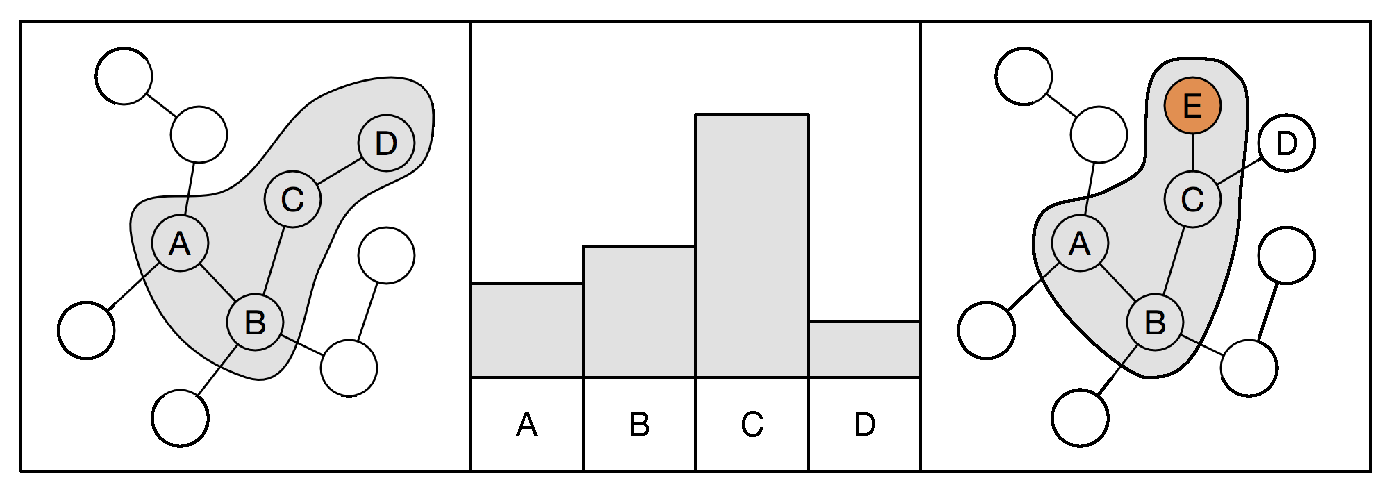
\includegraphics[scale=.5]{sf_add.eps}
\caption{The first pane shows a knowledge network, and a shaded region
  representing the active context. The second pane shows the memory accesses
  to particular items of knowledge leading up to the addition of a new item
  of knowledge. The third pane shows the new knowledge network, with the
  additional item of knowledge.}
\label{fig:sf_add}
\end{figure}

\begin{table}[h]
  \begin{center}
  \begin{tabular}{|l|p{4in}|}
    \hline
    {\tt Get() \{Item\}}  & Yields the set of items in the active context \\
                            \hline
    {\tt Add(Item)}       & Adds an item to the knowledge network \\ \hline
    {\tt Explore(ID)}     & Shifts context to focus on the item identified
                            by the given ID \\ \hline
    {\tt Connect(ID, ID)} & Forces the creation of an edge connecting the
                            two items of knowledge identified by the given
                            IDs \\
    \hline
  \end{tabular}
  \end{center}
\caption{Methods on an instance of the knowledge network.}
\label{tab:sf_get}
\end{table}


The SKN system implements a knowledge abstraction. The system is implemented
as an object with methods defining an interface, outlined in Table
\ref{tab:sf_get}, where {\tt Item} is a structure containing a unique
identifier, a symbolic tag denoting which mechanism can understand the
content, and the arbitrary content itself. The {\tt Add} method adds the given
item to the network based on least effort attachment according to the
frequency of memory accesses to knowledge items leading up to the addition,
illustrated in Figure \ref{fig:sf_add}. Only the {\tt Add} and {\tt Explore}
methods have the potential to augment the active context.

The context itself is of constant size in the asymptotic sense, in that it
may vary but not as a function of the size of the knowledge-base. The
sub-network of the context is also scale-free to allow for easy traversal of
both specialized and generally useful knowledge.


\section{Evaluation Metrics}

To experiment with SKN, consider the class of problems for which this system
would excel: complex domains where modular knowledge improves the efficiency
of completing relevant tasks. We augment a system for learning via iterative
modular concept discovery --- the EC algorithm \cite{dechter13} --- to
interface with SKN rather than use a flat set of knowledge items. The
augmented EC algorithm will be tested in the domains of letter analogies
\cite{hofstadter94}, L-systems \cite{rozenberg80}, and Boolean circuits
illustrated in Figure \ref{fig:exps}, and compared to the original EC algorithm in the as
well as a baseline of search without knowledge assistance. These problem
domains were chosen because they each have potential for common underlying
structure between tasks. Results will be compared on the number of tasks
solved given number of iterations for the algorithm.

\begin{figure}[h]
\centering
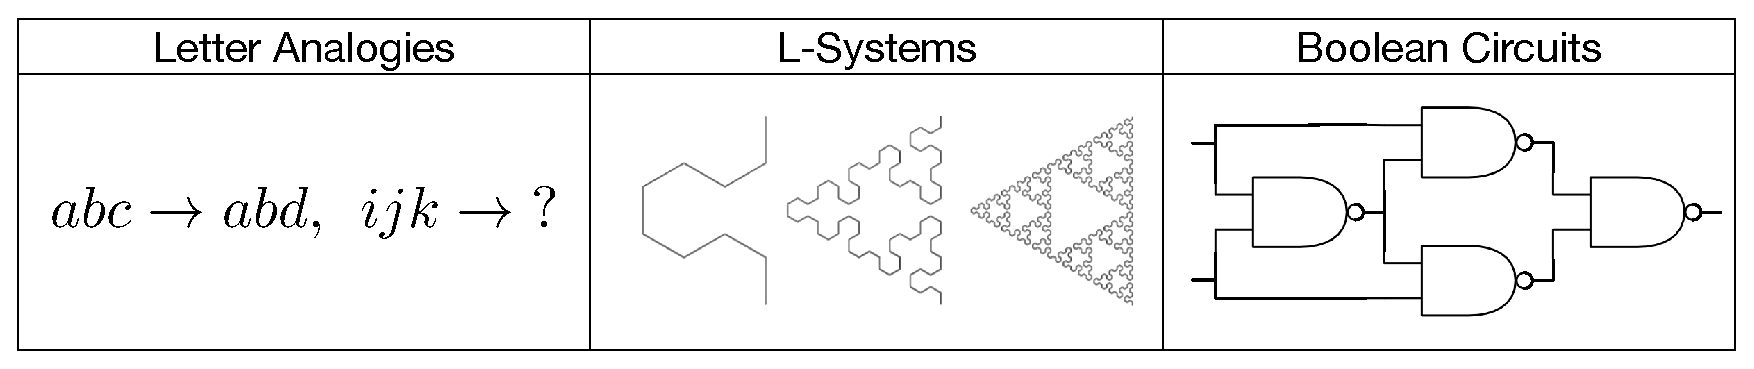
\includegraphics[scale=.5]{exps.eps}
\caption{Domains for test experiments.}
\label{fig:exps}
\end{figure}


\section{Conclusion}

We introduce SKN, a knowledge abstraction to improve learning mechanisms by
utilizing context in a scale-free network, with the purpose of better
modeling memory and knowledge in a convenient paradigm that fits both the
intuitive architecture of cognition and the programmatic methods of
computation that govern technology.


\section{Future Work}

The SKN system can be utilized in many different ways. By connecting many
learning mechanisms to the same knowledge network, interoperability between
distinct learning mechanisms such as vision and sound can result in proximal
--- and perhaps even shared --- items of knowledge representing the same
symbol being percieved by different mechanisms. Because learning mechanisms
treat abstract knowledge as first-class objects that can be observed,
modified, or created, the mechanisms don't necessarily have to be restricted
to \emph{learners} --- the introduction of \emph{actors} as mechanisms would
yield a powerful production system conditioned on contextual knowledge and
immediate circumstance. Supplemented with support for direct communication
between mechanisms, the mechanisms would be more fittingly referred to as
\emph{agents} \cite{minsky88}.


\section{Timeline}

\begin{itemize}
  \item September-October --- preliminary formalization, decide on
    experiments.
  \item November-January --- preliminary implementation, completed
    formalization.
  \item February --- finalize implementation.
  \item March-April --- complete paper writeup.
\end{itemize}


\begin{thebibliography}{}
  \bibitem{barabasi99}
    Barab\'asi, A. L., \& Albert, R. (1999).
    Emergence of scaling in random networks.
    \emph{Science}, 286(5439), 509-512.
  \bibitem{cancho03} i Cancho, R. F., \& Ricard V. Solé. (2003)
    Least effort and the origins of scaling in human language.
    In \emph{Proceedings of the National Academy of Sciences} 100(3), 788-791.
  \bibitem{zipf49} Zipf, G. K. (1949).
    Human Behaviour and the Principle of Least-Effort.
  \bibitem{clauset09} Clauset A., Shalizi, C. R., \& Newman M. E. J.  (2009)
    Power-law distributions in empirical data.
    \emph{SIAM Review} 51(4), 661-703 (arXiv:0706.1062, doi:10.1137/070710111)
  \bibitem{serre07}
    Serre, T., Oliva, A., \& Poggio, T. (2007).
    A feedforward architecture accounts for rapid categorization.
    In \emph{Proceedings of the National Academy of Sciences}, 104(15), 6424-6429.
  \bibitem{lake15} Lake, B. M., Salakhutdinov, R., \& Tenenbaum, J. B. (2015).
    Human-level concept learning through probabilistic program induction.
    \emph{Science}, 350(6266), 1332-1338.
  \bibitem{kulkarni15}
    Kulkarni, T. D., Whitney, W. F., Kohli, P., \& Tenenbaum, J. (2015).
    Deep convolutional inverse graphics network.
    In \emph{Advances in Neural Information Processing Systems} (pp. 2539-2547).
  \bibitem{mcdermott11}
    McDermott, J. H., \& Simoncelli, E. P. (2011).
    Sound texture perception via statistics of the auditory periphery:
    evidence from sound synthesis.
    \emph{Neuron}, 71(5), 926-940.
  \bibitem{tenenbaum01}
    Tenenbaum, J. B., \& Griffiths, T. L. (2001).
    The rational basis of representativeness.
    In \emph{Proceedings of the 23rd annual conference of the Cognitive
    Science Society} (p. 103641).
  \bibitem{liang10}
    Liang, P., Jordan, M. I., \& Klein, D. (2010).
    Learning programs: a hierarchical Bayesian approach.
    \emph{International Conference on Machine Learning}: 639–646
  \bibitem{dechter13}
    Dechter, E., Malmaud, J., Adams, R. P., \& Tenenbaum, J. B. (2013).
    Bootstrap Learning via Modular Concept Discovery.
    In \emph{IJCAI}.
  \bibitem{lavrac94}
    Lavrac, N., \& Dzeroski, S. (1994).
    Inductive Logic Programming.
    In \emph{WLP} (pp. 146-160).
  \bibitem{muggleton15}
    Muggleton, S. H., Lin, D., \& Tamaddoni-Nezhad, A. (2015).
    Meta-interpretive learning of higher-order dyadic datalog: Predicate
    invention revisited.
    \emph{Machine Learning}, 100(1), 49-73.
  \bibitem{goodfellow14}
    Goodfellow, I., Pouget-Abadie, J., Mirza, M., Xu, B., Warde-Farley, D.,
    Ozair, S., ... \& Bengio, Y. (2014).
    Generative adversarial nets.
    In \emph{Advances in Neural Information Processing Systems} (pp.
    2672-2680).
  \bibitem{anderson83}
    Anderson, J. R. (1983).
    \emph{The architecture of cognition}. Psychology Press.
  \bibitem{newell94}
    Newell, A. (1994).
    \emph{Unified theories of cognition}. Harvard University Press.
  \bibitem{hofstadter94}
    Hofstadter, D. R., \& Mitchell, M. (1994).
    The copycat project: A model of mental fluidity and analogy-making.
    \emph{Advances in connectionist and neural computation theory}, 2(31-112), 29-30.
  \bibitem{rozenberg80}
    Rozenberg, G., \& Salomaa, A. (1980).
    Mathematical Theory of L systems.
    \emph{Academic Press, Inc.}.
  \bibitem{minsky88}
    Minsky, M. (1988).
    \emph{Society of mind}.
    Simon and Schuster.
\end{thebibliography}

\end{document}
